% 1977 年江苏镇江地区初试卷第 9 题：三角形 ABC 中，D 在 AC 上（AD:DC=3:1），
% E 在 BC 上，AE 与 BD 相交于 G（BG=GD），按源卷第 3 页布局
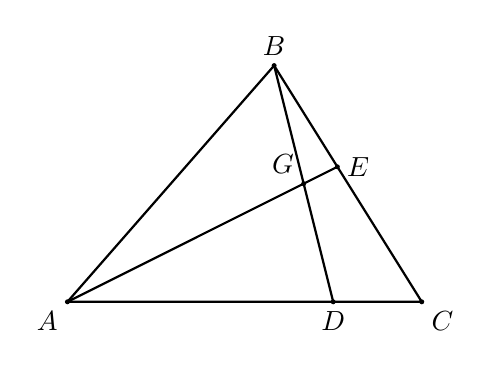
\begin{tikzpicture}[scale=0.75]
  \coordinate (A) at (0,0);
  \coordinate (C) at (6,0);
  \coordinate (B) at (3.5,4);
  \coordinate (D) at (4.5,0);
  \coordinate (E) at (4.571,2.286);
  \coordinate (G) at (4,2);
  \draw[thick] (A)--(B)--(C)--cycle;
  \draw[thick] (A)--(E);
  \draw[thick] (B)--(D);
  \fill (A) circle (1.2pt) node[below left] {$A$};
  \fill (B) circle (1.2pt) node[above] {$B$};
  \fill (C) circle (1.2pt) node[below right] {$C$};
  \fill (D) circle (1.2pt) node[below] {$D$};
  \fill (E) circle (1.2pt) node[right] {$E$};
  \fill (G) circle (1.2pt) node[above left] {$G$};
\end{tikzpicture}
